\documentclass{article}
\usepackage{amsmath}
\usepackage{tikz}
\usetikzlibrary{calc}

\begin{document}

\begin{figure}[h]
    \centering
    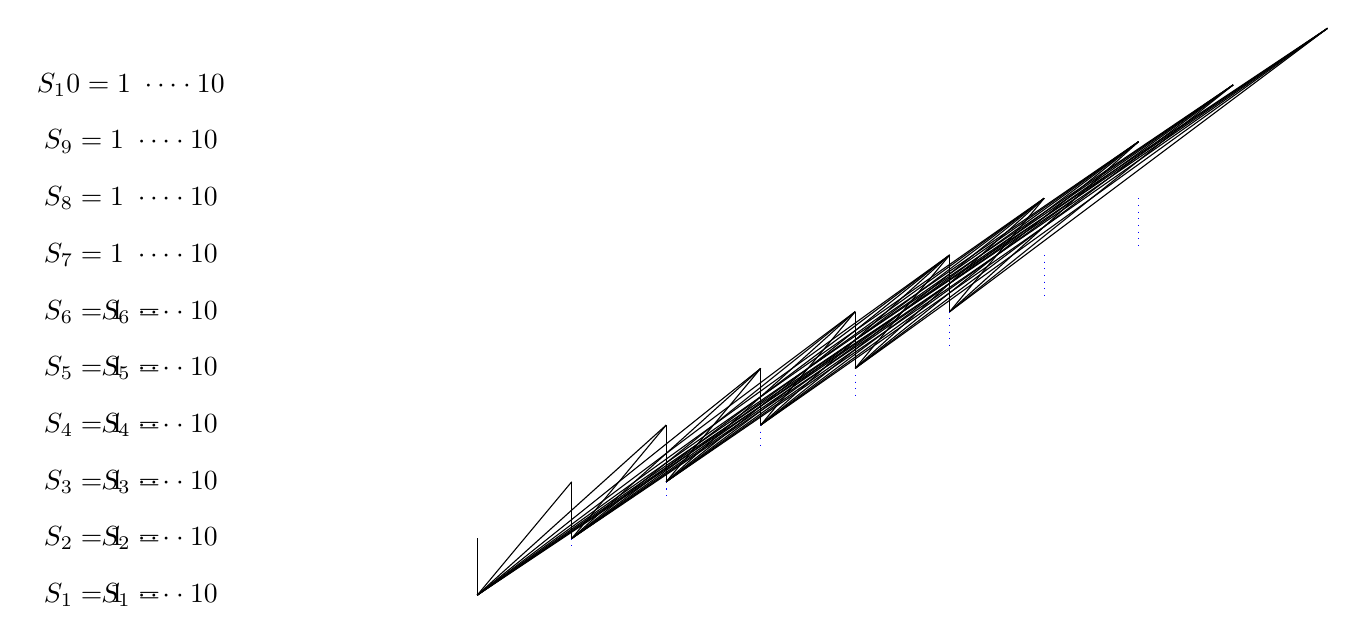
\begin{tikzpicture}[scale = 0.8]
        \foreach \j in {1,...,10} {
            \node at (-4,\j*.9) {$S_\j=1 \ \dotsm \cdot 10$};
        }
        \foreach \i [evaluate=\i as \ji using int(\i+1)] in {1,...,6} {
            \foreach \j [evaluate=\j as \kj using int(\j+1)] in {\i,...,10} {
                \draw (\i*1.5,\i*.9)--(\j*1.5,\kj*.9);
            }
            \node at (-4,\i*.9) {$S_\i=\jk$};
            \foreach \j [evaluate=\j as \kj using int(\j+1)] in {\i,...,\ji} {
                \draw[blue,dotted] (\kj*1.5,\kj*.9)--(\kj*1.5,\kj*.8);
            }
        }
    \end{tikzpicture}
    \caption{A diagram illustrating the sequence of $|\lambda_f|$ for all $f\in \mathcal{I}_2$ and $m=7$. The maximum value belongs to $x_5x_6$, which gives $|\lambda_{x_5x_6}|=2(m-2)=10$. The sequence of $S_j$ is symmetric: $1,1,2,2,3,3,3,2,2,1,1$.}
    \label{fig:sequence_Sj}
\end{figure}

\end{document}